\chapter{基于进化算法的FPGA脉动阵列快速硬核布局方法}



\section{问题建模}

本文将FPGA硬核布局建模为一个存在约束的多目标优化问题。首先,本文以Xilinx UltraScale+ VU11P FPGA举例说明异构FPGA中硬核的排布方法和
架构带来的布局约束条件,建立布局问题的背景;然后说明本文中布局问题的多个优化目标,以及根据优化目标和约束条件建立布局模型的方法。

图\ref{fig:architecture}展示了Xilinx UltraScale+系列VU11P FPGA的整体架构和放大后两个时钟域内部的硬核排布。首先,VU11P FPGA
由3个超逻辑域(Super Logic Region, SLR)构成,每个超逻辑域内的可编程器件构成和排布完全相同;其次,超逻辑域内包含三种硬核,分别是
DSP48E2, RAMB18, URAM288,每种硬核按列排布,但不同硬核列之间的分布却是无规则的;同时,三种硬核的大小不同:URAM288最大,RAMB18其次,
而DSP48E2最小。VU11P共有960个URAM288单元、4032个RAMB18单元,9216个DSP48单元,因此硬核的资源是不均衡的。
硬核列之间排布的不规则、硬核资源的不均衡和硬核大小本身的不同给布局带来了挑战:低质量的排布会造成部分计算单元内部连线过长,
导致整体设计时钟频率低,且可布线程度(Routability)降低导致布线失败。
另一方面,由于硬核之间为级联设计了专用的高速布线资源,所以硬核的布局存在约束:
\begin{itemize}
    \item 级联的硬核必须按从下(South)到上(North)的顺序排布,且不能跨超逻辑域(SLR)。
    \item 级联的DSP48E2与URAM288必须映射在相邻的两个Site上。
    \item 级联的RAMB18必须映射在距离1个Site的相邻两个位置上。
\end{itemize}


\begin{figure}[h]
	\centering
	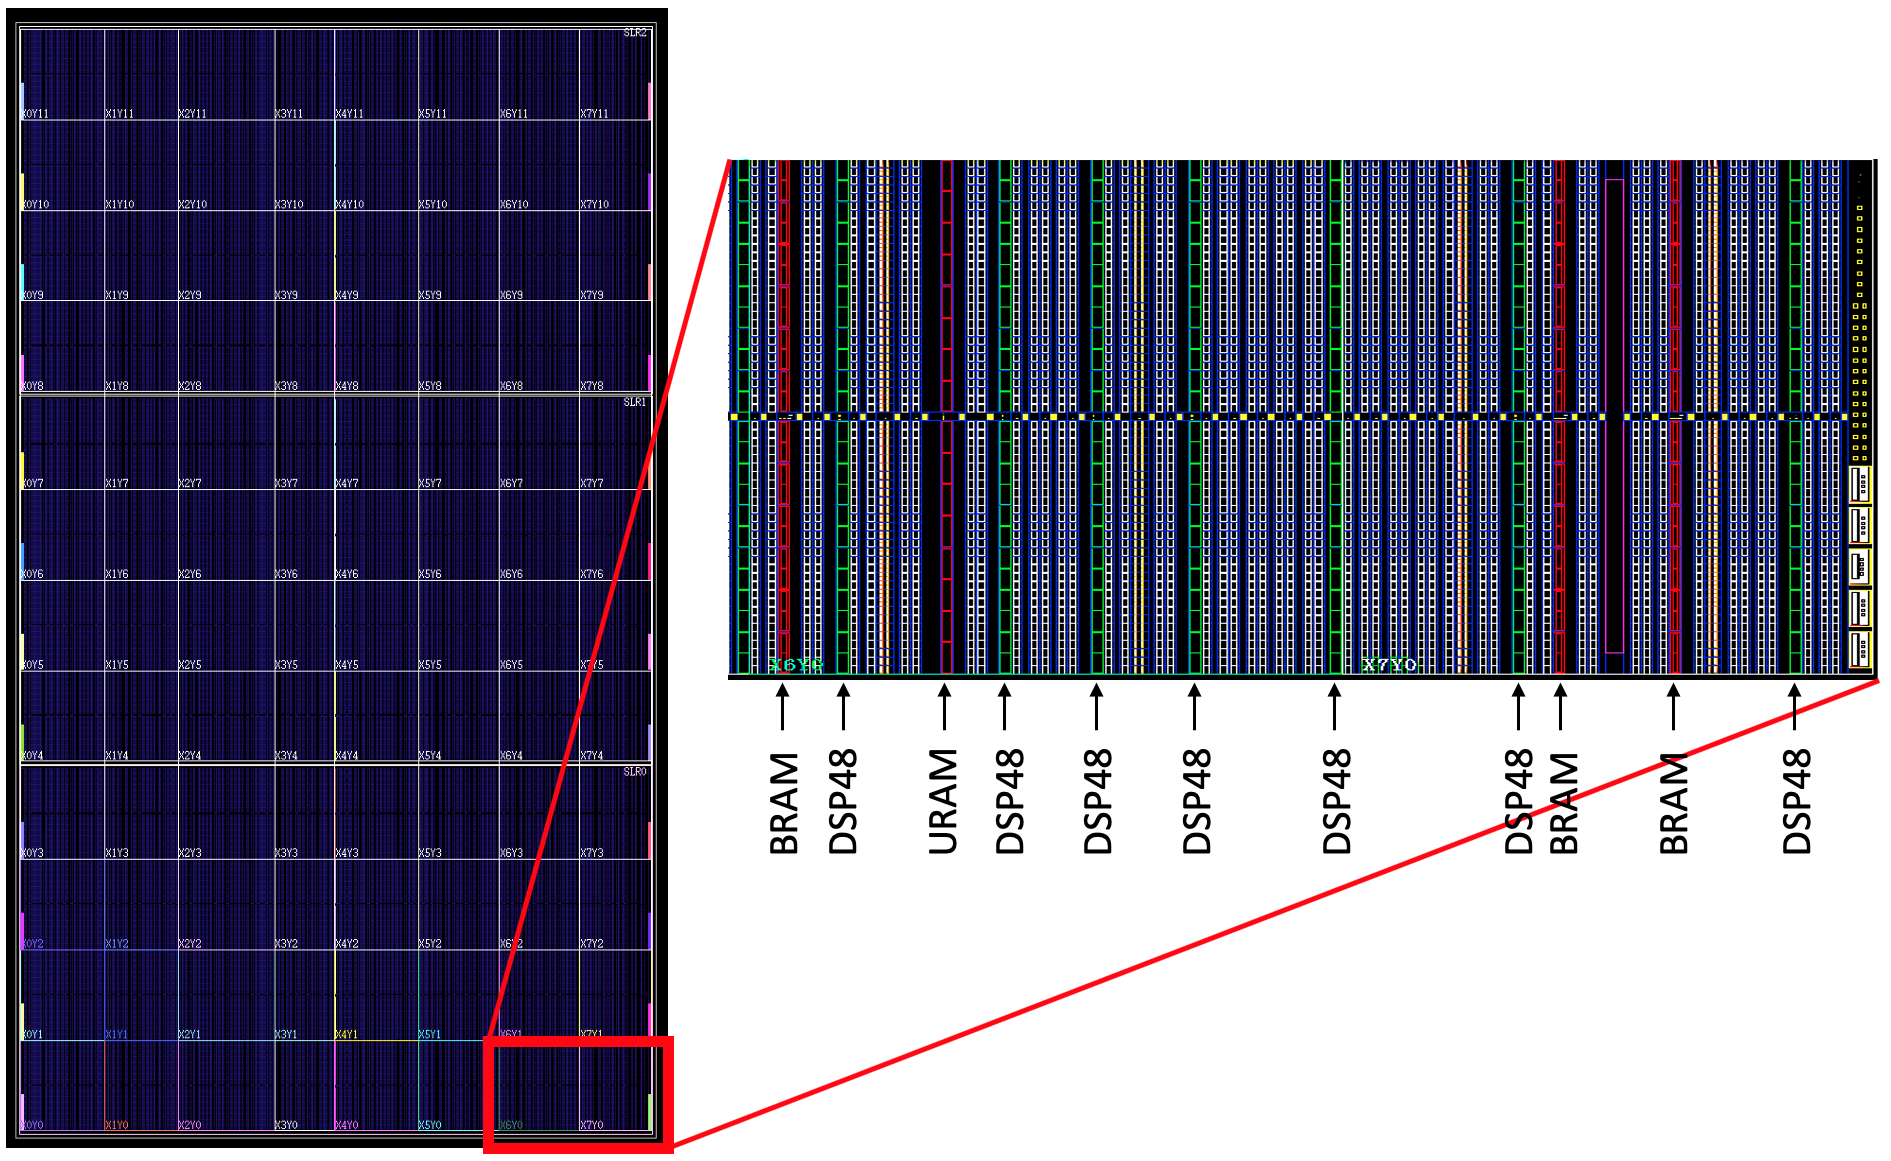
\includegraphics[width=\textwidth]{figure/architecture}
	\caption{Xilinx UltraScale+ VU11P 硬核列分布示意图} 
	\label{fig:architecture}
\end{figure}

FPGA布局的目的一般有两个:将Technology Mapping并分组后的逻辑网表映射到FPGA的物理器件上,保证设计可以布线;另一个目的是在可布线
的基础上追求小的延迟(delay),也就是尽可能短的关键路径(Critical Path)和尽可能高的时钟频率。因此,我们将硬核布局问题建立为一个
有约束的多目标优化问题:


\begin{equation} \label{eq:obj1}
	min \sum_{i,j} ((\Delta{x_{i,j}} + \Delta{y_{i,j}}) \cdot w_{i,j})^2 
\end{equation}

\begin{equation} \label{eq:obj2}
	 \min (\max_{k} BBoxSize(C_k))
\end{equation}

subject to:

% rectangle region bound
\begin{equation} \label{eq:region}
  0 \leq x_i,y_i < XMAX,YMAX
\end{equation}


% no overlap
\begin{equation} \label{eq:overlap}
    {x_i,y_i} \neq {x_j,y_j}
\end{equation}

% cascade connection placement requirement
\begin{equation} \label{eq:cascade}
  \begin{aligned}[b]
	& \textrm{if } i \textrm{ is cascaded after } j \textrm{ in the same column: }
  x_i = x_j \\
	& y_i =
	\begin{cases}
		 y_j + 1  & i, j \in \{  DSP, URAM  \} \\
		 y_j + 2  & i, j \in \{  RAMB \}
	\end{cases}
\end{aligned}
\end{equation}

在以上的等式中:
\begin{itemize}
	\item $i \in \{ DSP, RAM, URAM \} $ 表示逻辑网表映射到的FPGA上物理硬核单元。
	\item $C_k$ 表示卷积计算单元 $k$,其中包含2个URAM,18个DSP和8个BRAM。 
	\item $\Delta{x_{i,j}} + \Delta{y_{i,j}}$ 表示硬核$i$与硬核$j$之间的曼哈顿距离(Manhattan Distance)。
	\item $w_{i,j}$ 表示硬核$i$与硬核$j$之间距离的权重,这里我们用两个硬核之间连线的数目作为权重。
	\item $BBoxSize()$ 表示卷积核$C_k$的Bounding Box限制框尺寸,也就是限制框宽与高的和. 
	\item $x_i$ and $y_i$ 表示硬核$i$的RPM绝对坐标~\cite{ug903},用于计算两硬核之间的距离和卷积计算单元的限制框尺寸.
\end{itemize}

\subsection{布局问题的目标函数}
我们用线长的平方来表征布局的阻塞性能,如式\ref{eq:obj1},用最大限制框(Bounding Box)尺寸来表征卷积单元的关键路径(Critical Path)
如式\ref{eq:obj2}。这两个目标函数是紧密相关的,他们的目的在于同时尝试降低流水线寄存器消耗成本和提高时钟频率。
在实验中我们观察到,仅优化线长的平方会导致个别卷积运算单元收敛到横向长条形布局结果,导致关键路径出现在控制逻辑,时钟频率低且无法做流水线;
仅优化最大限制框尺寸,则会导致优化过程非常不稳定,容易收敛到局部最小值。因此,我们选择结合这两个目标函数来限制布局资源消耗同时追求
更高的时钟频率。

\subsection{布局问题的限制条件}
优化器仅需要遵守3个限制条件。(1)式\ref{eq:region}所表示的{\bf 区域限制条件}。它规定了布局优化所使用的硬核必须在FPGA上$XMAX \times YMAX$的
矩形区域内。(2)式\ref{eq:overlap}所表示的{\bf 非重合条件}。它用来防止优化器将多个逻辑硬核映射到同一个物理位置上。(3)式\ref{eq:cascade}所
表示的{\bf 级联条件},它规定了级联的硬核必须遵守Xilinx UltraScale+器件的布线规则。对于DSP和URAM,级联的两个硬核必须从下到上映射在两个
相邻的物理位置上。对于BRAM来说,级联的两个硬核必须从下到上映射到间隔一位的两个相邻物理位置上。BRAM映射规则的特殊性是由BRAM的类型决定的:
在UltraScale家族的器件中,块RAM (Block RAM)的基本类型是RAMB36,其内部包含两个RAMB18,分别是RAMB180和RAMB181。两种RAMB18都可以
使用,但是RAMB180仅能和RAMB180级联,RAMB181也仅能和RAMB181级联,这就造成了级联的RAMB18必须间隔一位放置。


\section{基于进化算法硬核布局的基因型设计}

\subsection{进化算法的基因型设计}

\begin{figure*}[t]
	\centering
	\resizebox{0.6\linewidth}{!}{
	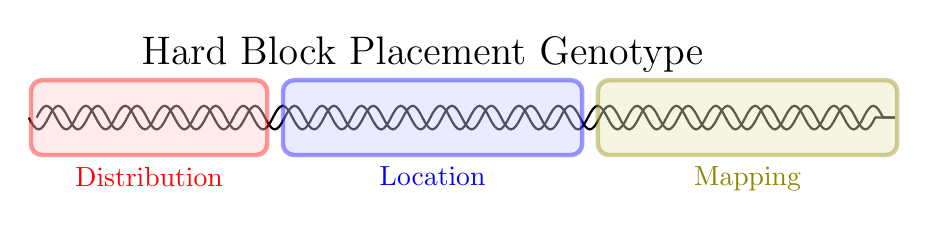
\begin{tikzpicture}[decoration={coil},
dna/.style={decorate, thick, decoration={aspect=0, segment length=0.5cm}}]
 
%DNA
	\draw[dna, decoration={amplitude=.15cm}] (.1,0) -- (11,0);
	\draw[dna, decoration={amplitude=-.15cm}] (0,0) -- (11,0);
	\node at (5,0.8) {\Large Hard Block Placement Genotype};

	\node [rectangle,rounded corners,inner sep=0pt,minimum width=3cm, minimum
  height=0.25cm,text height=0.95cm, draw=red, ultra thick, fill=red!20,
  anchor=west, opacity=0.4, text
  opacity=1,label=below:{\textcolor{red}{Distribution}}] at (0,0) {};

  \node [rectangle,rounded corners,inner sep=0pt,minimum width=3.8cm, minimum
  height=0.25cm,text height=0.95cm, draw=blue, ultra thick, fill=blue!20,
  anchor=west, opacity=0.4, text
  opacity=1,label=below:{\textcolor{blue}{Location}}] at (3.2,0) {};
 

	\node [rectangle,rounded corners,inner sep=0pt,minimum width=3.8cm, minimum
  height=0.25cm,text height=0.95cm, draw=olive, ultra thick, fill=olive!20,
  anchor=west, opacity=0.4, text
  opacity=1,label=below:{\textcolor{olive}{Mapping}}] at (7.2,0) {};
 
	\end{tikzpicture}
	
	}
	
	\subfloat[distribution]{
		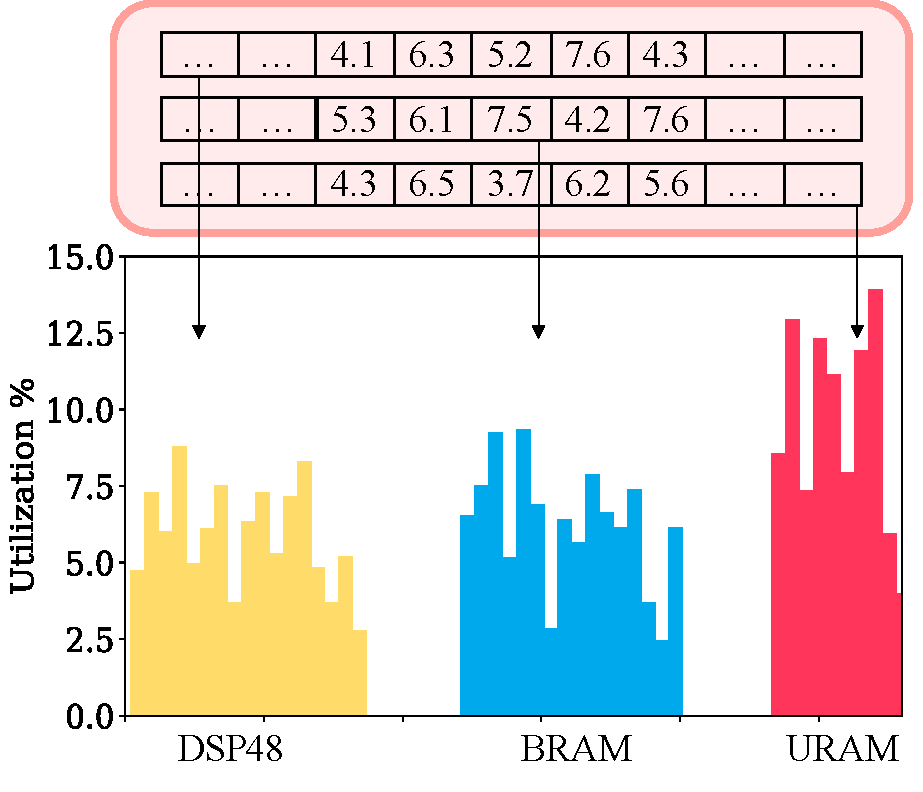
\includegraphics[width=0.30\textwidth, valign=t]{figure/geno-distribution.pdf}
		\vphantom{
			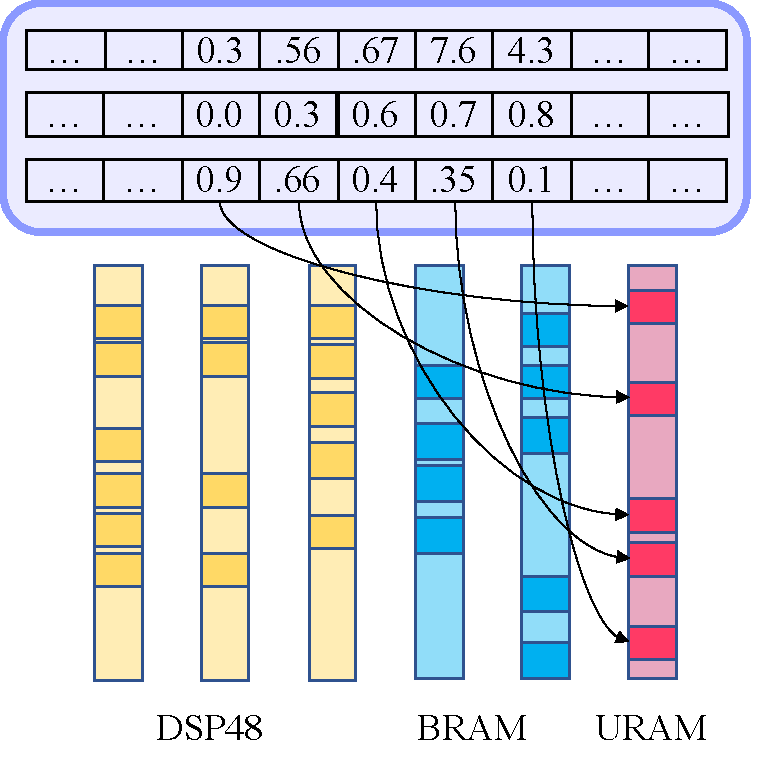
\includegraphics[width=0.25\textwidth, valign=t]{figure/geno-location.pdf}
			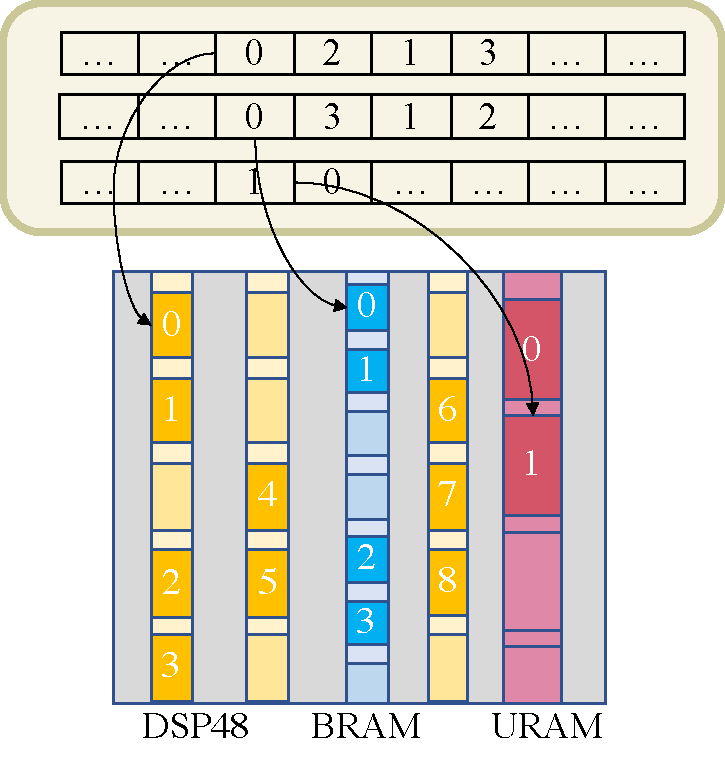
\includegraphics[width = 0.23\textwidth, valign=t]{figure/geno-mapping.pdf}
		}
	}
	\hfill
	\subfloat[location]{
		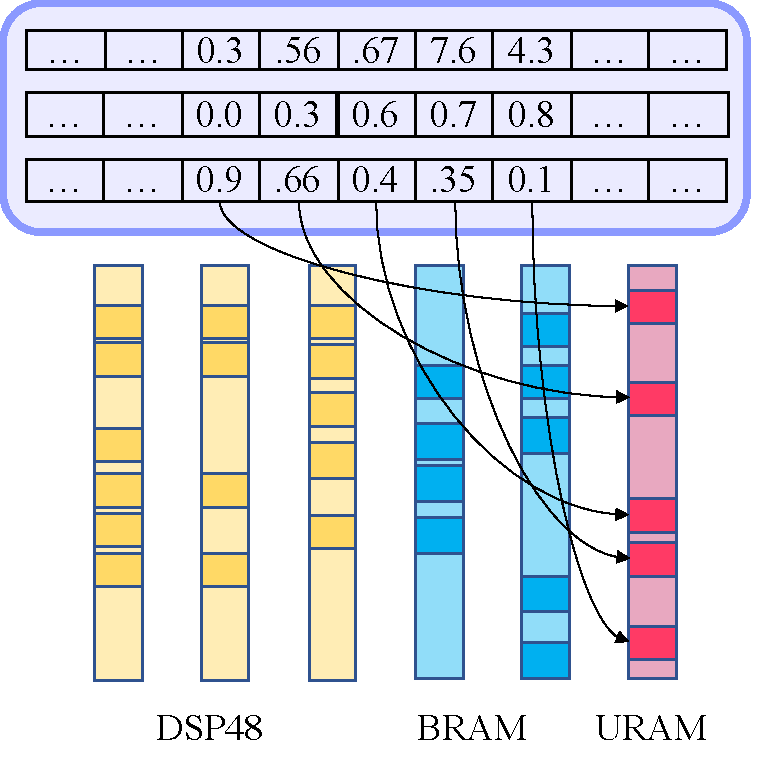
\includegraphics[width=0.25\textwidth, valign=t]{figure/geno-location.pdf}
		\vphantom{
			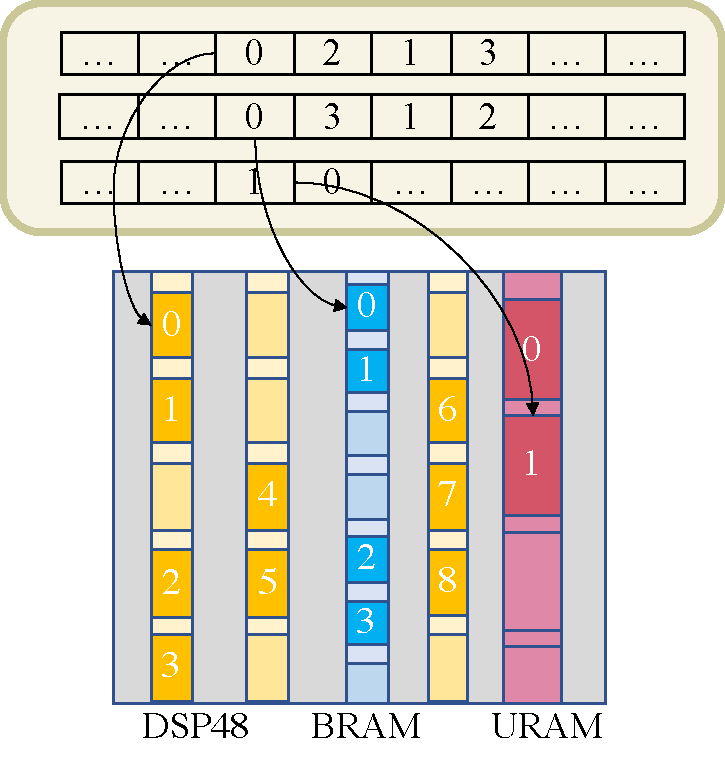
\includegraphics[width = 0.23\textwidth, valign=t]{figure/geno-mapping.pdf}
		}
	}
	\hfill
	\subfloat[mapping]{
		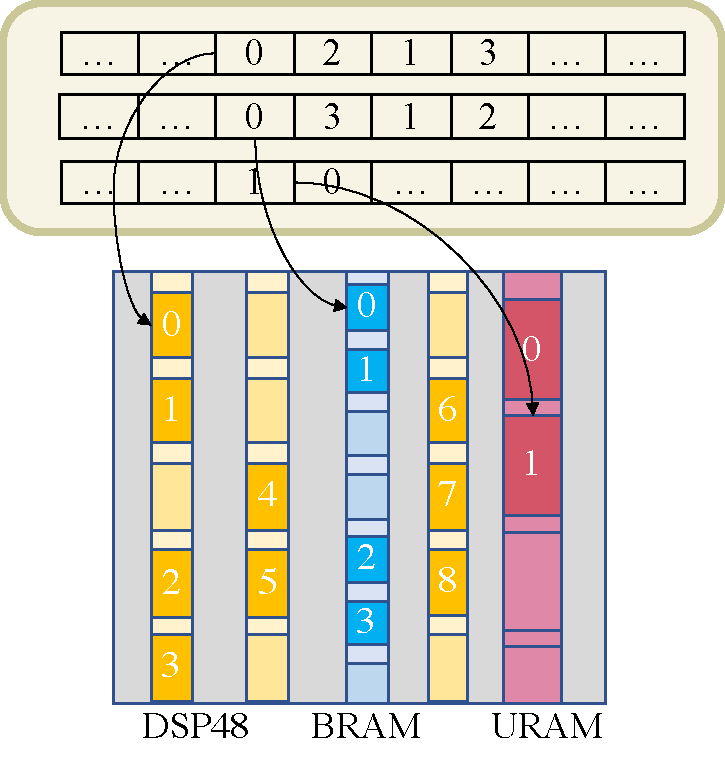
\includegraphics[width = 0.23\textwidth, valign=t]{figure/geno-mapping.pdf}
	}
	
	\caption{Our three-tier genotype design for hard block placement. 
	(a) Distribution defines the amount of hard blocks to be placed in each column. 
	(b) Location encodes the relative position of the corresponding hard blocks in its column. 
	(c) Mapping defines the connectivity of hard blocks, i.e., which hard blocks are mapped to one convolution unit. 
	The selected physical hard-block groups are numbered, which corresponds to the mapping genotype.
	}
	
	

	\label{fig:genotype}
  \vspace{-0.2in}
\end{figure*}

对于以上讨论的布局问题,K个卷积运算单元暴力搜索法需要尝试的问题空间大小在 $SP! \times BRAM! \times URAM! = 9K!\times4K!\times1K!$
的数量级,显然是行不通的。本文提出基于进化算法的应和布局,可以在短时间内发现高质量的布局结果。在进化算法中使用基因型来编码可行解,因此合理的
基因型设计对优化效果有至关重要的影响。我们将布局问题分解为三个子问题:硬核的列分布,硬核在列中的位置,硬核之间的连接关系。根据这三个子问题,我们
设计了对应的基因型。

\begin{itemize}
	\item \textcolor{red}{\bf Distribution} 因为卷积加速器设计中使用的各硬核比例不一定完全符合FPGA板上的硬核资源比例,
		又由于UltraScale系列硬件的硬核资源为按列分布,因此将使用的硬核资源按比例分配到各列,这一部分基因型就是规定了按什么样的比例
		将使用的硬核资源分配到各列。在解码该部分基因型时,首先将其归一化,然后根据归一化后的值和各列含有的硬核数目决定每一列放置
		多少个该种类硬核。
	\item \textcolor{blue}{\bf Location} 在我们决定了每一列放置硬核的数目之后,下一步需要决定的是硬核在每一列中的位置。
		这一部分基因型规定的就是每个硬核在该列的位置。此基因型使用 0$\rightarrow$1 浮点数对应硬核在列中从下到上的相对位置,
		也就是基因型中位置值接近0的硬核将被放置在列下方的位置,接近1的硬核将被放在列上方的位置。
	\item \textcolor{olive}{\bf Mapping} 最终,当确定了硬核放置的数目和位置之后,我们也就确定了在所有的物理硬核位置中,哪些
		硬核位置被选中用于布局。最终需要确定的,是将逻辑网表中的硬核映射到物理位置时候的对应关系。我们将选中的硬核位置编号,
		Mapping基因型中规定这些位置编号的排列,在解码时按顺序将基因型中的排列对应到网表中的硬核,这样就规定了逻辑网表中硬核
		到物理硬核的对应关系。这实际上影响的是每个卷积单元中硬核的连接关系。
\end{itemize}

以上说明的三种子基因型分别对应着布局问题的三个子问题,在图\ref{fig:genotype}中,我们对基因型设计进行了可视化。这三种子基因型
是紧密相关、互相依赖的,因此无法拆解为三个单独的问题分别优化。我们针对这一特性设计了一种 Composite Genotype 来适应子问题的
依赖关系,具体来说,三个子问题分别编码,在优化过程中分别更新,彼此之间不相互影响,但是在计算基因型的适应度函数 (Fitness Function)
的时候,三个子基因型一同解码计算。


\subsection{基因型解码时的解合法化}

为了适应浮点优化方法,我们通过解合法化 (Solution Legalization) 步骤对基因型采取量化等操作得到实际的布局,这一步骤在解码时进行。
算法 \ref{algo:distribution} 展示了了分布基因型的解码和合法化过程。由于假定可用资源已知,因此我们首先将分布量化为整数,
然后将每个整数值限制到每列的最大可放置硬核数。然后,我们将上一步去掉的硬核均匀分给其他的列。

\begin{algorithm}
	\SetKwFunction{GetDistribution}{GetDistribution}
	\SetKwFunction{Normalize}{Normalize}
	\SetKwFunction{GetMaxBlock}{GetMaxBlock}
	\SetKwFunction{Sum}{Sum}\SetKwFunction{Min}{Min}
	\SetKwFunction{Int}{Int}
	\SetKwInOut{Input}{input}\SetKwInOut{Output}{output}
	
	%\Input{Available hard block resources, distribution genotype}
	%\Output{Number of hard blocks to place for each column}
	%\BlankLine
	hardBlocks = \{DSP48, BRAM, URAM\}\;
	\ForEach {hardBlock in hardBlocks}{
		\tcp{distribution: a float array}
		distribution = \GetDistribution{hardBlock, genotype}\; 
		distribution = \Normalize{Distribution}\;
		\tcp{quantize}
		\For {$i\leftarrow 0$ \KwTo distribution.length}{
			distribution[i] = distribution[i] $\times$ blockSum\;
			distribution[i] = \Min{distribution[i], columnMax}\;
		}
		\tcp{handle rounding error}
		count=0\;
		\While{count $<$ blockSum - \Sum{distribution}}{
			col\_idx = 0\;
			\While{col\_idx $<$ all\_columns}{
				\If{ distribution[col\_idx] + 1 $\leq$ column\_max}{
					distribution[col\_idx] += 1\;
					count++\;
				}
				col\_idx++\;
				\If{count == block\_sum - \Sum{distribution}}{\textbf{break}\;}
			}
		}
		
   }

	\caption{Distribution genotype legalization}
	\label{algo:distribution}
\end{algorithm}

算法 \ref{algo:location} 展示了位置基因型的解码与合法化过程。
由于硬块位置是离散的,因此将对基因型中的连续值进行量化。
每个量化后的值都是级联链中第一个硬核的位置,所以从位置基因型直接解码的级联链位置可能会重叠或超出列中可用的硬核范围。
因此,我们对量化的位置进行排序,并从下至上调整位置。
位置调整首先检查可用的硬核是否足以放置该列剩余的级联链,如果不能则将当前级联链向下调整到所需位置,
来使超出范围的硬核放置合法化。
另一方面,如果当前组与前一组重叠,则将其调整为向上移动,直到合法放置为止。

\begin{algorithm}
	\SetKwFunction{GetLocation}{GetLocation}
	\SetKwFunction{Partition}{Partition}
	\SetKwFunction{Sort}{Sort}
	\SetKwFunction{Int}{Int}
	
	
	hardBlocks = \{DSP48, BRAM, URAM\}\;
	\ForEach {hardBlock in hardBlocks}{
		location = \GetLocation{hardBlock, genotype}\;
		\tcp{partition location into columns}
		location\_columns = \Partition{location, distribution}\;
		\ForEach {l\_column in location\_columns} {
			\Sort{l\_column, ascending}\;
			\For{$i\leftarrow 0$ \KwTo l\_column.length} {
				l\_column[i] $\times$= columnSize\;
				l\_column[i] = \Int{l\_column[i]}\;
				need = (l\_column.length-i-1) $\times$ group\_size\;
				avail = columnSize - (l\_column[i] + group\_size)\;
				\If{need $>$ avail}{l\_column[i] -= need - avail\;}
				\ElseIf{l\_column[i] $<$ l\_column[i-1] + group\_size}{
					l\_column[i] = l\_column[i-1] + group\_size\;
				}
			}
			
			
		}
	}
	
	\caption{Location genotype legalization}	
	\label{algo:location}
\end{algorithm}

由于Mapping基因型只优化编码的顺序,而不对编码的值进行修改,所以不会产生不合法编码,也就不需要解合法化。
以上内容详细阐述了解合法化的步骤,这些步骤保证了布局结果满足三个限制条件,并且与解析布局方法(Analytical Placement)
相比,我们的合法化步骤开销更低。



\section{布局框架工作流:RapidLayout Design Flow}


% figure: design flow

\tikzstyle{block} = [thick, rectangle, draw, fill=white, text width=12em, text centered, rounded corners, minimum height=2em]
\tikzstyle{invisiblock} = [rectangle, fill=white, text width=12em, text centered, rounded corners, minimum height=2em]
\tikzstyle{decisionblock} = [rectangle, draw, fill=blue!20, text width=12em, text centered, rounded corners, minimum height=2em]
\tikzstyle{line} = [draw, -latex']


\pgfdeclarelayer{bg}    % declare background layer
\pgfsetlayers{bg,main}  % set the order of the layers (main is the standard layer)


\begin{figure}
 \begin{center}
 \begin{tikzpicture}[node distance=1.5cm and 3.5cm, scale=1, transform shape]
   % Place nodes
   \node [invisiblock] (input) {Convolution Block DCP};
   \node [block, below of=input] (replicate) {Netlist Replication {\bf [\textless 1s]}};
   \circledat{A}{replicate.north west};
   \node [block, below of=replicate, minimum height=7em, node distance=2.5cm] (evolve) {Evolutionary\\ Hard Block\\ Placement\\ {\bf [30\,s--5\,min]}};
   \circledat{B}{evolve.north west};
   \node [block, below of=evolve, node distance=2.5cm] (siteroute) {Placement and\\ Site Routing {\bf [$\approx$3\,min]}};
   \circledat{C}{siteroute.north west};
   \node [block, below of=siteroute] (pipeline) {Post-Placement\\Pipelining {\bf [$\approx$10\,s]}};
   \circledat{D}{pipeline.north west};
   \node [block, below=0.75cm of pipeline] (vivado) {SLR Placement\\ and Routing {\bf [$\approx$54\,min]}};
   \circledat{E}{vivado.north west};
   \node [block, below=0.75cm of vivado] (slr) {SLR Replication {\bf [$\approx$2\,min]}};
   \circledat{F}{slr.north west};
   % Draw sub-nodes
  	 \node [block, fill=olive!50, right=1cm of evolve] (two) {Compute objective};
   \node [block, fill=olive!50, above of=two] (one) {Generate candidates};
   \node [block, fill=olive!50, below of=two] (three) {Update};
   % Inner loop highlight
   \begin{pgfonlayer}{bg}
   
   \path[rounded corners, draw=blue, thick, fill=blue!10,opacity=0.9] 
	([xshift=-0.75em,yshift=0.75em]vivado.north west) to ([xshift=10em,yshift=0.75em]vivado.north east) 
	to ([xshift=10em,yshift=-0.75em]vivado.south east) to ([xshift=-0.75em,yshift=-0.75em]vivado.south west) -- cycle;
   
   
   \path[rounded corners, draw=red, thick, fill=red!10,opacity=0.9] 
	([xshift=-0.75em,yshift=0.75em]replicate.north west) to 
 ([xshift=20em,yshift=0.75em]replicate.north east) to 
 ([xshift=20em,yshift=-0.75em]slr.south east) to
 ([xshift=-0.75em,yshift=-0.75em]slr.south west) to
 ([xshift=-0.75em,yshift=0.75em]slr.north west) to 
 ([xshift=12em,yshift=0.75em]slr.north east) to
	([xshift=12em,yshift=-0.75em]pipeline.south east) to 
 ([xshift=-0.75em,yshift=-0.75em]pipeline.south west) -- cycle;
   
   \path[rounded corners, draw=olive, thick, fill=olive!10,opacity=0.9] 
	([xshift=-0.5em,yshift=0.5em]evolve.north west) to ([xshift=0.5em,yshift=0.5em]evolve.north east) 
	to ([xshift=-0.5em,yshift=1.5em]one.north west) to ([xshift=3.5em,yshift=1.5em]one.north east) 
	to ([xshift=3.5em,yshift=-1.5em]three.south east) to ([xshift=-0.5em,yshift=-1.5em]three.south west) 
	to ([xshift=0.5em,yshift=-0.5em]evolve.south east) to ([xshift=-0.5em,yshift=-0.5em]evolve.south west) -- cycle;
   \end{pgfonlayer}
   
   %\node [draw=none,below right=0.1cm of three] (opt4j) {\bf Opt4J};
   \node [draw=none,right=3.5cm of slr] (RapidWright) {\Large \bf RapidWright};
   \node [draw=none,right=1.75cm of vivado] (RapidWright) {\Large \bf Vivado};
   
   \node [invisiblock,below of=slr] (output) {Bitstream};
   % Draw edges
   \path [line, thick] (input) -- (replicate);
   \path [line, thick] (replicate) -- (evolve);
   \path [line, thick] (evolve) -- (siteroute);
   \path [line, thick] (siteroute) -- (pipeline);
   \path [line, thick] (pipeline) -- (vivado);
   \path [line, thick] (vivado) -- (slr);
   \path [line, thick] (slr) -- (output);
   % Draw sub-edges
   \path [line, thick] (one) -- (two);
   \path [line, thick] (two) -- (three);
   % Loops
   \path [line, thick] (three.east) -- ([xshift=0.8cm]three.east) -- ([xshift=0.8cm]one.east) node [midway, above, sloped, rotate=180] (textnode0) {evolve} -- (one.east);

 \end{tikzpicture}
 \end{center}
	\caption{RapidLayout Design Flow with runtime details for the Xilinx VU11P
 FPGA along with tool usage information. Bulk of the intelligent exploration is done in RapidWright, and Vivado is only invoked at the end for final placement and routing.}
	\label{fig:flow}
 \vspace{-0.1in}
\end{figure}




\section{Example Walkthrough}













\section{本章小结}
















































% \chapter{几何驱动的用户目标区域提取与矫正方法}
% 内容概括 \cite{zhang98}。

% \section{勾画式用户目标区域标注}
% 勾画式用户标注,是一种简单易行的标注方法\cite{hariharan14,Li08,Su81,Liu93,jiang99} 。……

% \section{基于颜色聚类的目标区域提取方法}
% \label{sec1}
% 这里的颜色分类其实是为图像目标区域提取服务的。通过对图像颜色进行分类,结合用户的标注指定,我们得到用户期望的目标区域的颜色分类,根据这些分类就能够提取出颜色传递的目标区域。……

% \section{几何驱动的目标区域边界矫正方法}
% \ref{sec1} 节提出的目标区域提取方法可以在均匀性或一致性的前提下将图像目标物体或目标区域分割出来,若与相邻部分合并则会破坏这种一致性。

% \section{几何驱动的目标区域提取与矫正实验结果分析}
% 我们进行了图像目标区域提取与矫正实验。……

% \section{本章小结}
% 本章阐述了图像局部颜色编辑方法中图像目标区域提取的相关方法,……
